\section{Finite-Time Limitation of Exact Same-Point DC Criticality}
\label{Appendix: Finite-Time Barriers of DC}

\subsection{An explicit hard instance and the role of the DC oracle}
\label{subsec:explicit-dc-instance}

\citep{Zhang-2020-Complexity} prove that finding an \(\varepsilon\)-stationary point of a nonsmooth nonconvex Lipschitz function is impossible in finite time, and introduce \((\delta,\varepsilon)\)-stationarity as a relaxed target. We use their resisting-oracle construction. Our proof strategy is similar to Theorem 1.1.2 in (Nesterov, 2018) and Theorem 5 in \cite{Zhang-2020-Complexity}, where the resisting strategy is used to prove a lower bound.

% The DC setting departs from the smooth nonconvex setting in two ways that need to both be
% addressed on a single explicit instance, as discussed in the main text:
% the DC oracle is \emph{stronger}, since it can return the two component
% values $\phi(x),g(x)$ and the two component subgradients separately
% rather than a single generalized gradient of $F=\phi-g$; and the DC
% target is \emph{weaker}, since $0\in\partial\phi(x)-\partial g(x)$ is
% implied by, but does not imply, Clarke stationarity of $F$. A
% construction whose two component kink sets are disjoint proves the first
% point but not the second, because on such an instance
% $\partial\phi(x)-\partial g(x)=\partial_C F(x)$ everywhere and the DC
% target set never actually exceeds the Clarke target set. We therefore
% build the hard instance in two layers: a disjoint-kink \emph{background
% pair}, which forces every queried point to have DC residual bounded away
% from zero, and an \emph{invisible common-kink layer}, added identically
% to both convex components at a hidden location $s$, which is invisible
% to the strong oracle at every queried point yet creates a point that is
% DC-critical without being Clarke stationary. The two layers are combined
% into a proof of \Cref{thm:dc-oracle-limitation-sketch} in
% \Cref{subsec:main-proof} at the end of this appendix.

Throughout the appendix, let \(\{x^k\}_{k=1}^K\) be the chronological query sequence generated by the method and let
\(Q=\{x_1<\cdots<x_K\}\) denote these points sorted in ascending order (relabeling if necessary). We assume without loss of
generality (WLOG) that the initial point is queried and belongs to $Q$;
otherwise, one may query the initial point before running the algorithm.

\subsection{Background}
\label{subsec:background-pair}

We first recall the resisting instance at the level of the
weak transcript $(F(x),u(x)-v(x))$, which suffices to establish that
every queried point has DC residual bounded away from zero. Whenever the algorithm queries a point \(x\), the oracle returns
\[
    F(x)=0,\qquad
    u(x)\in\partial\phi(x),\qquad
    v(x)\in\partial g(x),
\]
chosen so that $u(x)-v(x)=L$. 
% The following lemma shows that this
% promise is realizable by a DC pair, for any finite query set, and
% that it in fact holds for a whole family indexed by a geometric
% parameter $\theta$; for the purposes of the strong-oracle argument below,
% we invoke it at a single fixed value $\theta=\theta_0\in(0,1/2)$ (e.g.\
% $\theta_0=1/4$) and do not use the family structure to hide information
% from the algorithm. Hiding under the strong oracle is instead the job of
% the common-kink layer constructed in \Cref{subsec:common-kink}: the
% family in $\theta$ is a \emph{geometry template}, not a \emph{hidden
% parameter}, once component values are observable.


\begin{lemma}
\label{lem:background-pair}
Given a finite sequence of real numbers
\(\{x_k\}_{k=1}^K\subset\mathbb R\), there exists a family of DC pairs
\(F_\theta=\phi_\theta-g_\theta\) such that, for any \(k\in[1,K]\),
\[
    F_\theta(x_k)=0,\qquad
    u_\theta(x_k)-v_\theta(x_k)=L,
    \quad
    u_\theta(x_k)\in\partial\phi_\theta(x_k),\
    v_\theta(x_k)\in\partial g_\theta(x_k).
\]
Moreover, for sufficiently small \(\varepsilon<L\), the DC
\(\varepsilon\)-critical sets of two different choices of \(\theta\) can be
chosen disjoint.
\end{lemma} 

\begin{figure}[t]
\centering
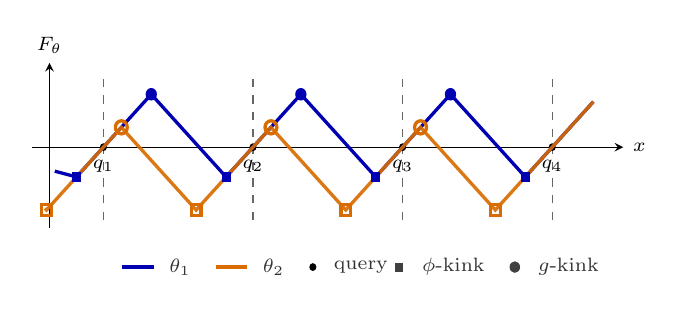
\begin{tikzpicture}[
    >=stealth,
    font=\scriptsize,
    xscale=0.95,
    yscale=1.05,
    query/.style={black!60, dashed, thin},
    thetaone/.style={blue!70!black, very thick},
    thetatwo/.style={orange!85!black, very thick},
    phione/.style={blue!70!black},
    gone/.style={blue!70!black},
    phitwo/.style={orange!85!black},
    gtwo/.style={orange!85!black},
    legendtext/.style={black!80},
]

% ------------------------------------------------------------
% Drawing parameters:
% q_k = 0,2,4,6, delta = 2.
% theta_1 = 0.18, theta_2 = 0.38.
% a_k(theta)=q_k-theta*delta, b_k(theta)=(q_k+q_{k+1})/2-theta*delta.
% ------------------------------------------------------------

% Axes
\draw[->] (-0.95,0) -- (6.95,0) node[right] {$x$};
\draw[->] (-0.72,-0.98) -- (-0.72,1.02) node[above] {$F_\theta$};

% Query points: shared by both theta values
\foreach \x/\lab in {0/$q_1$,2/$q_2$,4/$q_3$,6/$q_4$}{
    \draw[query] (\x,-0.88) -- (\x,0.88);
    \fill[black] (\x,0) circle (1.35pt);
    \node[below] at (\x,-0.04) {\lab};
}

% theta_1 curve, theta_1*delta=0.36
\draw[thetaone]
    (-0.65,-0.29) --
    (-0.36,-0.36) --
    (0,0) --
    (0.64,0.64) --
    (1.64,-0.36) --
    (2,0) --
    (2.64,0.64) --
    (3.64,-0.36) --
    (4,0) --
    (4.64,0.64) --
    (5.64,-0.36) --
    (6,0) --
    (6.55,0.55);

% theta_2 curve, theta_2*delta=0.76
\draw[thetatwo, opacity=0.92]
    (-0.78,-0.74) --
    (-0.76,-0.76) --
    (0,0) --
    (0.24,0.24) --
    (1.24,-0.76) --
    (2,0) --
    (2.24,0.24) --
    (3.24,-0.76) --
    (4,0) --
    (4.24,0.24) --
    (5.24,-0.76) --
    (6,0) --
    (6.55,0.55);

% theta_1 phi-side kinks: squares
\foreach \x/\y in {-0.36/-0.36,1.64/-0.36,3.64/-0.36,5.64/-0.36}{
    \fill[phione] (\x,\y) ++(-0.06,-0.06) rectangle ++(0.12,0.12);
}

% theta_1 g-side kinks: circles
\foreach \x/\y in {0.64/0.64,2.64/0.64,4.64/0.64}{
    \fill[gone] (\x,\y) circle (2.15pt);
}

% theta_2 phi-side kinks: hollow-ish squares
\foreach \x/\y in {-0.76/-0.76,1.24/-0.76,3.24/-0.76,5.24/-0.76}{
    \draw[phitwo, very thick] (\x,\y) ++(-0.065,-0.065) rectangle ++(0.13,0.13);
}

% theta_2 g-side kinks: hollow-ish circles
\foreach \x/\y in {0.24/0.24,2.24/0.24,4.24/0.24}{
    \draw[gtwo, very thick] (\x,\y) circle (2.25pt);
}

% Legend below the plot
\begin{scope}[shift={(0.25,-1.45)}]
    \draw[thetaone] (0,0) -- (0.42,0);
    \node[legendtext, anchor=west] at (0.50,0) {\(\theta_1\)};

    \draw[thetatwo] (1.25,0) -- (1.67,0);
    \node[legendtext, anchor=west] at (1.75,0) {\(\theta_2\)};

    \fill[black] (2.55,0) circle (1.35pt);
    \node[legendtext, anchor=west] at (2.70,0) {query};

    \fill[black!75] (3.70,0) ++(-0.055,-0.055) rectangle ++(0.11,0.11);
    \node[legendtext, anchor=west] at (3.88,0) {\(\phi\)-kink};

    \fill[black!75] (5.25,0) circle (2.0pt);
    \node[legendtext, anchor=west] at (5.43,0) {\(g\)-kink};
\end{scope}

\end{tikzpicture}
\vspace{0.55em}
\caption{
DC resisting family. Distinct hidden shifts \(\theta\) preserve the same query transcript \(F(q_k)=0,\ u_k-v_k=L\).
}
\label{fig:dc-resisting-family}
\end{figure}

\begin{proof}
Without loss of generality, we assume $x_1<x_2<\cdots<x_K$, reordering the
indices if necessary. We construct $F_\theta=\phi_\theta-g_\theta$ as a
family of sawtooth functions and show that it simultaneously satisfies the
resisting-transcript property and the disjointness of $\varepsilon$-critical
sets.

Let
\[
    \delta
    =
    \min\limits\left\{
    \min\limits_{k\in[1,K-1]}(x_{k+1}-x_k),\
    \frac{\Delta}{L}
    \right\},
\]
with the first term omitted when $K=1$. For $\theta\in(0,1/2)$, define
\[
    a_k(\theta)=x_k-\theta\delta,\quad k\in[1,K],
    \qquad
    b_k(\theta)=\frac{x_k+x_{k+1}}2-\theta\delta,\quad k\in[1,K-1],
\]
and set $\alpha_\theta=Lx_1-2L\theta\delta$. We define the two convex
components by
\[
    \phi_\theta(x)=\alpha_\theta-Lx+2L\sum_{k=1}^{K}(x-a_k(\theta))_+,
    \qquad
    g_\theta(x)=2L\sum_{k=1}^{K-1}(x-b_k(\theta))_+ .
\]
Since $(\cdot)_+$ is convex and all hinge coefficients above are
nonnegative, $\phi_\theta$ and $g_\theta$ are proper, closed, convex,
piecewise-linear functions, with kinks located at $\{a_k(\theta)\}_{k=1}^K$
and $\{b_k(\theta)\}_{k=1}^{K-1}$, respectively (see
Figure~\ref{fig:dc-components}).

\begin{figure}[t]
\centering
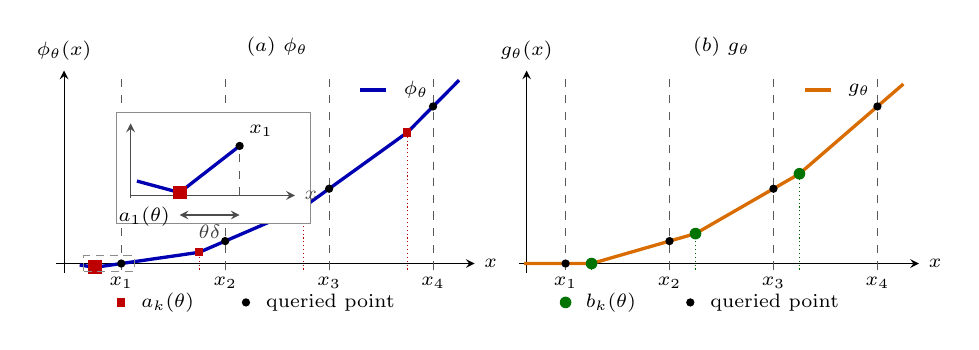
\begin{tikzpicture}[
    >=stealth,
    font=\scriptsize,
    xscale=0.66,
    yscale=0.095,
    query/.style={black!65, dashed, thin},
    philine/.style={red!70!black, densely dotted, thin},
    gline/.style={green!40!black, densely dotted, thin},
    phicurve/.style={blue!70!black, very thick},
    gcurve/.style={orange!85!black, very thick},
    insetbox/.style={draw=black!45, fill=white, line width=0.3pt},
    insetnote/.style={black!75},
    querymark/.style={circle, fill=black, inner sep=0pt, minimum size=3pt},
    phimark/.style={rectangle, fill=red!75!black, inner sep=0pt, minimum size=3pt},
    phifirst/.style={rectangle, fill=red!75!black, inner sep=0pt, minimum size=5pt},
    gmark/.style={circle, fill=green!45!black, inner sep=0pt, minimum size=4.2pt},
]

% Representative drawing parameters:
% L=1, x_k=0,2,4,6, delta=2, theta=1/4.
% Hence a_k(theta)=-0.5,1.5,3.5,5.5 and
% b_k(theta)=0.5,2.5,4.5.

% ===================== phi panel =====================
\node[anchor=south] at (3.0,26.4) {\((a)\) \(\phi_\theta\)};
\draw[->] (-1.25,0) -- (6.8,0) node[right] {$x$};
\draw[->] (-1.1,-1.2) -- (-1.1,25.8) node[above] {$\phi_\theta(x)$};

\foreach \x/\lab in {0/$x_1$,2/$x_2$,4/$x_3$,6/$x_4$}{
    \draw[query] (\x,-0.8) -- (\x,24.7);
    \node[below] at (\x,-0.55) {\lab};
}
\foreach \x/\y in {-0.5/-0.5,1.5/1.5,3.5/7.5,5.5/17.5}{
    \draw[philine] (\x,-0.8) -- (\x,\y);
}
\draw[phicurve]
    (-0.8,-0.2) --
    (-0.5,-0.5) --
    (0,0) --
    (1.5,1.5) --
    (2,3) --
    (3.5,7.5) --
    (4,10) --
    (5.5,17.5) --
    (6,21) --
    (6.5,24.5);
\foreach \x/\y in {1.5/1.5,3.5/7.5,5.5/17.5}{
    \node[phimark] at (\x,\y) {};
}
\node[phifirst] at (-0.5,-0.5) {};
\foreach \x/\y in {0/0,2/3,4/10,6/21}{
    \node[querymark] at (\x,\y) {};
}
\draw[black!45, densely dashed] (-0.72,-1.05) rectangle (0.25,1.05);
\begin{scope}[shift={(0.18,9.1)}, xscale=1.52, yscale=7.7]
    \draw[insetbox] (-0.18,-0.48) rectangle (2.28,1.45);
    \draw[->, black!70] (0,0) -- (2.08,0) node[right] {$x$};
    \draw[->, black!70] (0,-0.04) -- (0,1.25);
    \draw[phicurve]
        (0.08,0.25) --
        (0.62,0.05) --
        (1.38,0.86);
    \node[phifirst] at (0.62,0.05) {};
    \node[querymark] at (1.38,0.86) {};
    \draw[philine] (0.62,0) -- (0.62,0.05);
    \draw[query] (1.38,0) -- (1.38,0.86);
    \node[below left] at (0.62,-0.03) {$a_1(\theta)$};
    \node[above right] at (1.38,0.86) {$x_1$};
    \draw[<->, black!70, thin] (0.62,-0.34) -- (1.38,-0.34)
        node[midway, below, insetnote] {$\theta\delta$};
\end{scope}
\draw[phicurve] (4.6,23.2) -- (5.1,23.2);
\node[anchor=west] at (5.25,23.2) {$\phi_\theta$};
\node[phimark] at (0.0,-5.2) {};
\node[anchor=west] at (0.2,-5.2) {$a_k(\theta)$};
\node[querymark] at (2.4,-5.2) {};
\node[anchor=west] at (2.6,-5.2) {queried point};

% ===================== g panel =====================
\begin{scope}[xshift=8.55cm]
\node[anchor=south] at (3.0,26.4) {\((b)\) \(g_\theta\)};
\draw[->] (-0.9,0) -- (6.8,0) node[right] {$x$};
\draw[->] (-0.75,-1.2) -- (-0.75,25.8) node[above] {$g_\theta(x)$};

\foreach \x/\lab in {0/$x_1$,2/$x_2$,4/$x_3$,6/$x_4$}{
    \draw[query] (\x,-0.8) -- (\x,24.7);
    \node[below] at (\x,-0.55) {\lab};
}
\foreach \x/\y in {0.5/0,2.5/4,4.5/12}{
    \draw[gline] (\x,-0.8) -- (\x,\y);
}
\draw[gcurve]
    (-0.8,0) --
    (0.5,0) --
    (2,3) --
    (2.5,4) --
    (4,10) --
    (4.5,12) --
    (6,21) --
    (6.5,24);
\foreach \x/\y in {0.5/0,2.5/4,4.5/12}{
    \node[gmark] at (\x,\y) {};
}
\foreach \x/\y in {0/0,2/3,4/10,6/21}{
    \node[querymark] at (\x,\y) {};
}
\draw[gcurve] (4.6,23.2) -- (5.1,23.2);
\node[anchor=west] at (5.25,23.2) {$g_\theta$};
\node[gmark] at (0.0,-5.2) {};
\node[anchor=west] at (0.2,-5.2) {$b_k(\theta)$};
\node[querymark] at (2.4,-5.2) {};
\node[anchor=west] at (2.6,-5.2) {queried point};
\end{scope}

\end{tikzpicture}
\vspace{0.35em}
\caption{
Illustration of the two convex components \(\phi_\theta\) and \(g_\theta\),
drawn in separate panels to avoid overplotting.
The representative parameters are \(L=1\), \(x_k\in\{0,2,4,6\}\),
\(\delta=2\), and \(\theta=1/4\). The kinks of \(\phi_\theta\) occur at
\(a_k(\theta)\), the kinks of \(g_\theta\) occur at \(b_k(\theta)\), and the
two components agree at the queried points \(x_k\).
}
\label{fig:dc-components}
\end{figure}


By construction, the breakpoints interlace as
\[
    a_k(\theta)<x_k<b_k(\theta)<a_{k+1}(\theta)<x_{k+1},
    \qquad k\in[1,K-1],
\]
so that exactly $k$ kinks of $\phi_\theta$ and $k-1$ kinks of $g_\theta$
precede the query point $x_k$. Consequently,
\[
    \phi_\theta'(x_k)=(2k-1)L,
    \qquad
    g_\theta'(x_k)=2(k-1)L,
\]
and therefore
\[
    \phi_\theta'(x_k)-g_\theta'(x_k)=L
    \qquad\text{for every } k\in[1,K],
\]
independently of $k$. Setting $u_\theta(x_k)=\phi_\theta'(x_k)$ and
$v_\theta(x_k)=g_\theta'(x_k)$ therefore realizes the claimed resisting
transcript.

We now verify that $F_\theta(x_k)=0$ for every $k\in[1,K]$. Expanding the
hinge terms active at $x_k$ gives
\[
\begin{aligned}
F_\theta(x_k)
&=
\alpha_\theta-Lx_k
+2L\sum_{j=1}^{k}(x_k-a_j(\theta))
-2L\sum_{j=1}^{k-1}(x_k-b_j(\theta)) \\
&=
\alpha_\theta-Lx_1+2L\theta\delta
=
0,
\end{aligned}
\]
where the second equality follows by telescoping the interlacing
differences $a_j(\theta)-b_j(\theta)$ and $b_j(\theta)-a_{j+1}(\theta)$, and
the last equality holds by the choice of $\alpha_\theta$. Together with the
preceding display, this shows that the oracle returns the identical
transcript $\bigl(F_\theta(x_k),\,u_\theta(x_k)-v_\theta(x_k)\bigr)=(0,L)$ at
every query point, for every $\theta\in(0,1/2)$.

It remains to characterize the $\varepsilon$-critical set of $F_\theta$
and establish its disjointness across $\theta$. Away from the kinks,
$F_\theta'=\phi_\theta'-g_\theta'\in\{-L,L\}$ by the same interlacing
argument, so $F_\theta$ is $L$-Lipschitz. Moreover, since
$\operatorname{kink}(\phi_\theta)\cap\operatorname{kink}(g_\theta)=\emptyset$,
no cancellation occurs in the subdifferential of the sum, and
\[
    \partial\phi_\theta(x)-\partial g_\theta(x)=\partial_C F_\theta(x),
    \qquad\forall x\in\mathbb R .
\]
Since $\operatorname{dist}\bigl(0,\partial_C F_\theta(x)\bigr)=L$ at every
non-kink point, it follows that for any $\varepsilon<L$ the
$\varepsilon$-critical set coincides exactly with the kink set,
\[
    \mathcal S_\theta^\varepsilon
    =
    \{a_k(\theta):k\in[1,K]\}
    \cup
    \{b_k(\theta):k\in[1,K-1]\} .
\]
By definition, every element of $\mathcal S_\theta^\varepsilon$ equals a
$\theta$-independent quantity minus $\theta\delta$; that is,
$\mathcal S_\theta^\varepsilon$ is a rigid translate, by $-\theta\delta$, of
a fixed configuration determined solely by $\{x_k\}_{k=1}^K$. Since
$\theta\mapsto\theta\delta$ is injective on $(0,1/2)$, it follows that
$\mathcal S_{\theta_1}^\varepsilon\cap\mathcal S_{\theta_2}^\varepsilon
=\emptyset$ whenever $\theta_1\neq\theta_2$, which completes the proof.
\end{proof}

\begin{corollary}[Affine tail of the DC pair]
\label{cor:affine-tail}
Fix $\theta=\theta_0\in(0,1/2)$ and write $(\phi_0,g_0):=(\phi_{\theta_0},g_{\theta_0})$ for the pair of \Cref{lem:background-pair}. Then $\phi_0,g_0$ are affine on $[x_K,\infty)$, with
\[
    \phi_0'(x)=(2K-1)L,
    \qquad
    g_0'(x)=2(K-1)L,
    \qquad
    x\ge x_K,
\]
so that $u_0-v_0:=\phi_0'(x)-g_0'(x)=L$ throughout this ray.
\end{corollary}

\begin{proof}
By the interlacing $a_k(\theta_0)<x_k<b_k(\theta_0)<a_{k+1}(\theta_0)<x_{k+1}$
established in the proof of \Cref{lem:background-pair}, the largest kink
of $\phi_0$ is $a_K(\theta_0)<x_K$ and the largest kink of $g_0$ is
$b_{K-1}(\theta_0)<a_K(\theta_0)<x_K$. Hence both components are affine on
$[x_K,\infty)$, with slopes equal to the values computed at $x_K$ in the
proof of \Cref{lem:background-pair}.
\end{proof}

\subsection{Invisible common kink under the strong oracle}
\label{subsec:common-kink}

The DC pair of \Cref{lem:background-pair} was designed so that
its \emph{difference} $F_0=\phi_0-g_0$ carries no information about
$\theta_0$ at the queried points, which suffices under the weak oracle
$(F,u,v)$. Under the strong oracle $(\phi,g,\partial\phi,\partial g)$,
however, $\phi_0(x_k)$ and $g_0(x_k)$ are each individually informative:
querying two points on the affine tail of \Cref{cor:affine-tail} reveals
the intercept of $\phi_0$, and hence $\theta_0$, directly. We therefore
introduce a second layer whose hidden parameter is a \emph{location}
rather than a slope offset, and which is invisible to the strong oracle
by construction.

\begin{lemma}[Invisible common kink]
\label{lem:common-kink}
Let $(\phi_0,g_0)$ be affine on $[x_K,\infty)$ with slopes $u_0,v_0$
there. Fix $M>0$, $\beta\in\mathbb R$, and a hidden location $s>x_K$.
Define
\[
    c_s(x)=M|x-s|+\beta-Ms,
    \qquad
    \phi_s:=\phi_0+c_s,
    \qquad
    g_s:=g_0+c_s.
\]
Then $\phi_s,g_s$ are proper, closed, convex, and:
\begin{enumerate}
\item[\textup{(i)}] \textbf{Objective invariance.} $\phi_s-g_s=\phi_0-g_0$ everywhere.
In particular the Lipschitz constant of $\phi_s-g_s$, its optimality gap
$(\phi_s-g_s)(\bx^0)-\inf\limits_x(\phi_s-g_s)(x)$, and its Clarke subdifferential
$\partial_C(\phi_s-g_s)(x)$ at every $x$ are all independent of $s$.
\item[\textup{(ii)}] \textbf{Invisibility at queried points.} For every
$x\le x_K$,
\[
    c_s(x)=\beta-Mx,
    \qquad
    \partial c_s(x)=\{-M\},
\]
independent of $s$. Consequently, for every admissible $s>x_K$,
\[
    \phi_s(x_k)=\phi_0(x_k)+\beta-Mx_k,
    \quad
    g_s(x_k)=g_0(x_k)+\beta-Mx_k,
    \quad
    \partial\phi_s(x_k)=\partial\phi_0(x_k)-M,
    \quad
    \partial g_s(x_k)=\partial g_0(x_k)-M,
\]
none of which depends on $s$. In particular the DC residual at each
queried point equals the background residual,
$\operatorname{dist}(0,\partial\phi_s(x_k)-\partial g_s(x_k))
=\operatorname{dist}(0,\partial\phi_0(x_k)-\partial g_0(x_k))$.
\item[\textup{(iii)}] \textbf{Spurious DC-criticality at $s$.} At $x=s$,
\[
    \partial\phi_s(s)-\partial g_s(s)
    =
    \{u_0-v_0\}+M[-1,1]-M[-1,1]
    =
    \{u_0-v_0\}+[-2M,2M].
\]
If $M\ge|u_0-v_0|/2$, then $0\in\partial\phi_s(s)-\partial g_s(s)$. Since
$\partial_C(\phi_s-g_s)(s)=\{u_0-v_0\}$ by (i) and the affineness of
$\phi_0-g_0$ at $s$, we have $0\notin\partial_C(\phi_s-g_s)(s)$ whenever
$u_0\ne v_0$.
\end{enumerate}
\end{lemma}

\begin{figure}[t]
\centering
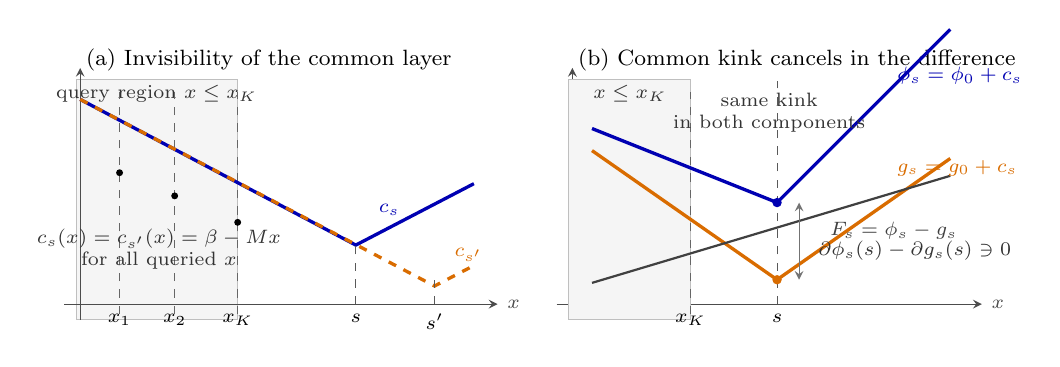
\begin{tikzpicture}[
    >=stealth,
    font=\scriptsize,
    axis/.style={black!70, thin, ->},
    query/.style={black!60, dashed, thin},
    hidden/.style={black!65, dashed, thin},
    csline/.style={blue!70!black, very thick},
    csp/.style={orange!85!black, very thick, dashed},
    phicurve/.style={blue!70!black, very thick},
    gcurve/.style={orange!85!black, very thick},
    fcurve/.style={black!75, thick},
    region/.style={fill=black!4, draw=black!25},
    legendtext/.style={black!80}
]

% Left panel: hidden locations are identical on the query region.
\begin{scope}
    \node[anchor=west, font=\footnotesize] at (0,3.45) {(a) Invisibility of the common layer};
    \draw[region] (0,0.15) rectangle (2.05,3.2);
    \node[legendtext] at (1.02,3.02) {query region \(x\le x_K\)};
    \draw[axis] (-0.15,0.35) -- (5.35,0.35) node[right] {$x$};
    \draw[axis] (0.05,0.15) -- (0.05,3.35);

    \foreach \x/\lab in {0.55/$x_1$,1.25/$x_2$,2.05/$x_K$}{
        \draw[query] (\x,0.22) -- (\x,3.05);
        \fill[black] (\x,2.25-0.42*\x) circle (1.25pt);
        \node[below] at (\x,0.35) {\lab};
    }

    \draw[csline]
        (0.05,2.95) -- (3.55,1.10) -- (5.05,1.88);
    \draw[csp]
        (0.05,2.95) -- (4.55,0.58) -- (5.05,0.84);

    \draw[hidden] (3.55,0.35) -- (3.55,1.18);
    \draw[hidden] (4.55,0.35) -- (4.55,0.66);
    \node[below] at (3.55,0.35) {$s$};
    \node[below] at (4.55,0.35) {$s'$};

    \node[blue!70!black, anchor=west] at (3.72,1.55) {$c_s$};
    \node[orange!85!black, anchor=west] at (4.68,0.98) {$c_{s'}$};
    \node[legendtext, align=center] at (1.05,1.05)
        {\(c_s(x)=c_{s'}(x)=\beta-Mx\)\\for all queried \(x\)};
\end{scope}

% Right panel: adding the same kink to both components creates DC criticality
% without changing the difference.
\begin{scope}[shift={(6.25,0)}]
    \node[anchor=west, font=\footnotesize] at (0,3.45) {(b) Common kink cancels in the difference};
    \draw[axis] (-0.15,0.35) -- (5.25,0.35) node[right] {$x$};
    \draw[axis] (0.05,0.15) -- (0.05,3.35);

    \draw[region] (0,0.15) rectangle (1.55,3.2);
    \node[legendtext] at (0.78,3.02) {\(x\le x_K\)};
    \draw[query] (1.55,0.22) -- (1.55,3.05);
    \node[below] at (1.55,0.35) {$x_K$};

    \draw[hidden] (2.65,0.35) -- (2.65,3.18);
    \node[below] at (2.65,0.35) {$s$};

    \draw[phicurve]
        (0.30,2.58) -- (2.65,1.64) -- (4.85,3.84);
    \draw[gcurve]
        (0.30,2.30) -- (2.65,0.66) -- (4.85,2.20);
    \draw[fcurve]
        (0.30,0.62) -- (4.85,1.98);

    \fill[blue!70!black] (2.65,1.64) circle (1.7pt);
    \fill[orange!85!black] (2.65,0.66) circle (1.7pt);
    \node[blue!70!black, anchor=west] at (4.05,3.25) {$\phi_s=\phi_0+c_s$};
    \node[orange!85!black, anchor=west] at (4.05,2.08) {$g_s=g_0+c_s$};
    \node[black!75, anchor=west] at (3.20,1.28) {$F_s=\phi_s-g_s$};

    \draw[<->, black!55] (2.93,0.66) -- (2.93,1.64);
    \node[legendtext, anchor=west] at (3.05,1.03)
        {\(\partial\phi_s(s)-\partial g_s(s)\ni0\)};
    \node[legendtext, align=center] at (2.55,2.78)
        {same kink\\in both components};
\end{scope}

\end{tikzpicture}
\vspace{0.4em}
\caption{
Invisible common-kink construction. Panel (a) shows that different hidden
locations \(s,s'>x_K\) induce the same values and subgradients on all queried
points \(x\le x_K\). Panel (b) shows that adding the same V-shaped layer to
both convex components creates a common kink at \(s\), while the objective
difference \(F_s=\phi_s-g_s\) remains unchanged and has no Clarke kink there.
}
\label{fig:invisible-common-kink}
\end{figure}

\begin{proof}
\textup{(i)} Immediate from $\phi_s-g_s=(\phi_0+c_s)-(g_0+c_s)=\phi_0-g_0$.

\textup{(ii)} For $x\le x_K<s$ we have $|x-s|=s-x$, so
\[
    c_s(x)=M(s-x)+\beta-Ms=\beta-Mx,
\]
which does not involve $s$; differentiating gives $\partial c_s(x)=\{-M\}$
on this ray. The displayed identities follow by adding $c_s$ (respectively
its subgradient) to $\phi_0,g_0$ (respectively $\partial\phi_0,\partial
g_0$) at $x_k$. The residual identity holds because subtracting the same
constant $-M$ from both $\partial\phi_0(x_k)$ and $\partial g_0(x_k)$
leaves their Minkowski difference, and hence its distance to $0$,
unchanged.

\textup{(iii)} Since $\phi_0,g_0$ are affine at $s>x_K$ with slopes
$u_0,v_0$ and $c_s$ has a kink at $s$ with $\partial c_s(s)=M[-1,1]$, the
subdifferential sum rule gives $\partial\phi_s(s)=\{u_0\}+M[-1,1]$ and
$\partial g_s(s)=\{v_0\}+M[-1,1]$; their Minkowski difference is
$\{u_0-v_0\}+[-2M,2M]$, which contains $0$ once $M\ge|u_0-v_0|/2$. The
Clarke-subdifferential claim follows from (i), since $\phi_0-g_0$ is
affine, hence smooth, at $s$.
\end{proof}

\subsection{Strong-transcript reduction}
\label{subsec:reduction}

\begin{lemma}[Strong-transcript reduction]
\label{lem:strong-reduction}
Let $(\phi_0,g_0)$, $M$, and $\beta$ be as in \Cref{lem:common-kink}, and
let $s,s'>x_K$ with $s\neq s'$. Let $(\phi_s,g_s)$ and $(\phi_{s'},g_{s'})$
be the corresponding pairs. Then:
\begin{enumerate}
\item[\textup{(i)}] The two instances return an identical strong-oracle
transcript at $x_1,\ldots,x_K$:
\[
    \bigl(\phi_s(x_k),g_s(x_k),\partial\phi_s(x_k),\partial g_s(x_k)\bigr)
    =
    \bigl(\phi_{s'}(x_k),g_{s'}(x_k),\partial\phi_{s'}(x_k),\partial g_{s'}(x_k)\bigr),
    \qquad
    k=1,\ldots,K.
\]
\item[\textup{(ii)}] Consequently, a deterministic algorithm interacting
with $\mathcal O_{\rm DC}$ produces the same query sequence
$x_1,\ldots,x_K$ against both instances; a randomized algorithm does so
as well when conditioned on its internal randomness.
\item[\textup{(iii)}] The two spurious critical points $s,s'$ are
distinct, and by \Cref{lem:common-kink}(ii), neither instance has an
$\varepsilon$-critical point among $x_1,\ldots,x_K$ once $\varepsilon<L$.
\end{enumerate}
Consequently, no algorithm making $K$ queries under $\mathcal O_{\rm DC}$
can guarantee, on both instances simultaneously, that some queried point
is $\varepsilon$-critical. Following the same two-instance,
disjoint-target argument used by \citet[Theorem~5]{Zhang-2020-Complexity}
(and reproduced for the $\theta$-family in \Cref{lem:background-pair}),
its success probability against the uniform mixture over $\{s,s'\}$ is at
most $1/2$.
\end{lemma}

\begin{proof}
Part (i) is \Cref{lem:common-kink}(ii) applied to both $s$ and $s'$. Part
(ii) holds because the algorithm's next query is a (possibly randomized)
function of the oracle responses observed so far; if these coincide at
every step for the two instances, so does the induced distribution over
query sequences. Part (iii) follows from $s\neq s'$ together with
\Cref{lem:common-kink}(ii)--(iii). The final probability bound follows
the identical-transcript, disjoint-target reduction already used to
separate $\mathcal S_{\theta_1}^\varepsilon$ from
$\mathcal S_{\theta_2}^\varepsilon$ in the proof of
\Cref{lem:background-pair}, applied here with the singleton target sets
$\{s\}$ and $\{s'\}$.
\end{proof}

\subsection{Proof of \Cref{thm:dc-oracle-limitation-sketch}}
\label{subsec:main-proof}

\begin{proof}[Proof of \Cref{thm:dc-oracle-limitation-sketch}]
Let $x_1<\cdots<x_K$ denote the (possibly random) points queried by the
algorithm. Fix $\theta_0\in(0,1/2)$, e.g.\ $\theta_0=1/4$, and let
$(\phi_0,g_0)$ be the disjoint-kink background pair of
\Cref{lem:background-pair} at $\theta=\theta_0$; by
\Cref{cor:affine-tail} it is affine on $[x_K,\infty)$ with slope gap
$u_0-v_0=L$. Set $M=L/2$, fix any $\beta\in\mathbb R$, and choose two
admissible locations $x_K<s<s'$, e.g.\ $s=x_K+1$, $s'=x_K+2$. Form
$(\phi_s,g_s)$ and $(\phi_{s'},g_{s'})$ as in \Cref{lem:common-kink}.

\emph{Class membership.} By \Cref{lem:common-kink}(i), the Lipschitz
constant and optimality gap of $\phi_s-g_s$ (resp.\ $\phi_{s'}-g_{s'}$)
equal those of $\phi_0-g_0$, which lie within $\Delta,L$ by construction
of the background pair. The component subgradient bound increases by at
most $M$ over the background bound $O(KL)$ established in
\Cref{lem:background-pair}'s proof, giving $G_K=O(KL+M)=O(KL)$; choosing
the constant $c$ in $K\le cG/L$ small enough ensures $G_K\le G$, so both
instances lie in $\mathcal D(\Delta,L,G)$.

\emph{Failure at queried points.} By \Cref{lem:common-kink}(ii), every
queried point $x_k$ has DC residual exactly $L>\varepsilon$ on both
instances.

\emph{Spurious DC-critical point.} By \Cref{lem:common-kink}(iii), with
$M=L/2$ the instance $(\phi_s,g_s)$ contains a point $s$ with
$0\in\partial\phi_s(s)-\partial g_s(s)$ and $0\notin\partial_C(\phi_s-g_s)(s)$,
and likewise $(\phi_{s'},g_{s'})$ contains such a point at $s'$.

\emph{Indistinguishability and the probability bound.} By
\Cref{lem:strong-reduction}, the two instances are indistinguishable to
the algorithm at every one of its $K$ queries, and no algorithm can
guarantee success against both simultaneously. Hence, with probability at
least $1/2$, the realized instance is one on which none of the first $K$
queried points is $\varepsilon$-critical, and this instance carries its
own spurious DC-critical, non-Clarke-stationary point. This proves the
theorem.
\end{proof}
